\subsubsection{Pumpen}
\label{subsubsec:Pumpen}

Um die Flüssigkeiten sauber befördern zu können, werden Vakuummembranpumpen eingesetzt. Diese werden oft in der Lebensmittelindustie verwendet, da diese einerseits hygienisch sind und zum andern einen guten Durchfluss bieten können. Ein weiterer Vorteil dieser Pumpen ist, dass durch die Erstellung eines Vakuums auch Luft gepumpt werden kann. Dies ermöglicht auch einen \flqq Kaltstart\frqq\ ohne Flüssigkeit in den Schläuchen. \cite{aiyimaindustrial_store_us_nodate}

\paragraph{Schema}\mbox{}

Die Schaltung zur Ansteuerung der Pumpen ist relativ simpel aufgebaut und in Abbildung \ref{fig:Schema_Pumpenansteuerung} zu sehen. Sie besteht aus einer kleinen Leistungsstufe, welche mit einem Logik-MOSFET realisiert wurde, welcher die 12V für die Pumpen  ein- und ausschaltet. Ausserdem beinhaltet die Schaltung einen Begrenzungswiderstand, eine Freilaufdiode und einen Stecker für den Anschluss der Pumpe. Die Schaltung wurde für alle zwölf Pumpen umgesetzt. \cite{aiyimaindustrial_store_us_nodate}

\begin{figure}[h!]
	\centering
	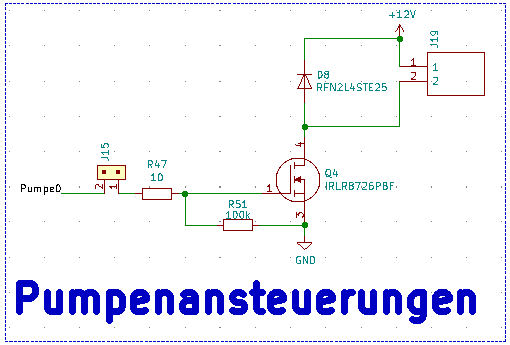
\includegraphics[width=0.5\textwidth]{graphics/Schema_Pumpenansteuerung.png}
	\caption{Schema der Pumpenansteuerung.}
	\label{fig:Schema_Pumpenansteuerung}
\end{figure}

\paragraph{Funktionsbeschrieb der Schaltung}\mbox{}

Die Pumpen werden jeweils direkt über den Mikrocontroller angesteuert. Dabei wird für jede Pumpe ein Digitalpin gemäss \ref{subsec:Mikrocontroller} verwendet. Da der Mikrocontroller nicht genügend Ausgangsstrom bietet, um die Pumpen ansteuern zu können, wurde eine kleine Leistungsstufe mit einem MOSFET (hier Q4) implementiert gemäss Abbildung \ref{fig:Schema_Pumpenansteuerung}. Es handelt sich bei diesem MOSFET um einen Logik-Level-Mosfet IRLR8726 von Infineon Technologies. Dieser hat den Vorteil, dass er direkt über einen Mikrocontroller angesteuert werden kann und trotz niedrigem Spannungsniveau voll durchsteuern kann. Da das Gate jedes MOSFET's auch eine Kapazität darstellt, wird der Anfangsstrom beim Einschalten des Pin's durch einen 10Ohm (hier R47) Widerstand begrenzt. Ein weiterer Grund für diesen Widerstand ist, dass manche MOSFET's beim Ein- und Auschalten, mit der steilen Flanke dazu neigen kurzzeitig zu oszillieren. Dies wird durch diesen Widerstand auch unterdrückt. Zu Messzwecken wurde vor diesem Widerstand ein Jumper implementiert. Dies ermöglicht es die Ansteuerung vom Mikrocontroller abzukoppeln. Da es sich bei dieser Pumpe um einem DC-Motor und somit um eine Induktion handelt, wurde parallel zur Pumpe am Stecker eine Freilaufdiode implementiert. Diese schützt den MOSFET vor Spannungsspitzen beim Ausschalten. \cite[S.362]{atmel_atmel_2014} \cite{aiyimaindustrial_store_us_nodate} \cite{mouser_mp24943dn-lf_nodate}